\documentclass[12pt]{article}
\usepackage[spanish]{babel}
\usepackage{geometry}
\usepackage{graphicx}
\usepackage{setspace}
\usepackage{hyperref}
\usepackage{apacite}
\usepackage{fancyhdr}
\usepackage{titlesec}
\usepackage{nopageno}
\usepackage{tocloft}


%  small letter size for title 12fnt
%     key words in the footer
% Justification lins
% only marco teorico and metodologia and anexos, encuesta/resultados
\geometry{a4paper, margin=1in}
\doublespacing
\title{\large{\textbf{AquaSolar: Sistema de Riego Sostenible para Huertas}}}
\author{Juan Andrés Del Toro R, Nathan Daniel Alspaugh y Juan Pablo Ortiz \\ Medio Ambiente, Colegio Real Royal School \\ Undecimo Grado \\ Lic. Corina Corpas Santofimio \\ 21 de Mayo de 2025}
\date{}
\begin{document}
\pagestyle{fancy}
\cfoot{}
\fancyhead{} % clear all header fields
\fancyhead[LO,CE]{\textbf{AquaSolar:  Sistema de Riego Sostenible para Huertas
      }}
\fancyhead[RO,RO]{\thepage}
\maketitle

\newpage
\renewcommand{\thesection}{}
\renewcommand{\thesubsection}{}
\renewcommand{\thesubsubsection}{}
\renewcommand{\cftsecleader}{\cftdotfill{\cftdotsep}}
\titleformat{\section} % Command to modify
{\normalfont\Large\bfseries} % Font style for the section title
{\thesection} % Section number (optional)
{0pt} % Space between number and title
{} % Code before the title (optional)

% Customize subsection formatting
\titleformat{\subsection} % Command to modify
{\normalfont\large\bfseries} % Font style for the subsection title
{\thesubsection} % Subsection number (optional)
{1em} % Space between number and title
{} % Code before the title (optional)

% Customize subsubsection formatting
\titleformat{\subsubsection} % Command to modify
{\normalfont\normalsize\bfseries} % Font style for the subsubsection title
{\thesubsubsection} % Subsubsection number (optional)
{2em} % Space between number and title
{} % Code before the title (optional)
\newpage
\section*{Resumen}
A lo largo de la historia, la humanidad ha enfrentado retos en la gestión de los recursos naturales, particularmente en el uso de fuentes de energía no renovables. Según la Agencia Internacional de Energía \cite{IEA2020}, la sobreexplotación de recursos como la electricidad, proveniente de fuentes fósiles, representa un desafío creciente para la sostenibilidad global. En este contexto, es urgente buscar soluciones sostenibles que promuevan el uso de energías limpias. El proyecto Aqua Solar responde a esta necesidad mediante la implementación de un sistema de riego automatizado que aprovecha la energía solar como fuente principal.

El objetivo central del proyecto es diseñar un sistema de riego eficiente, impulsado por energía solar, para huertos escolares, con el fin de reducir costos operativos, maximizar la utilización de energía, y fomentar la sostenibilidad ambiental. Al integrar paneles fotovoltaicos en el sistema, se garantiza la autosuficiencia energética, eliminando la dependencia de fuentes no renovables y promoviendo el uso de energía limpia. Además, el proyecto incluye un controlador automático que ajusta el riego según las necesidades específicas de las plantas, mejorando la gestión eficiente del agua.

Con este enfoque, el proyecto no solo busca optimizar el uso de la energía solar, sino también sensibilizar a los estudiantes sobre la importancia de las energías renovables y su impacto positivo en el medio ambiente.
\\~\\
\textbf{Palabras clave:} Energías limpias, energía solar, energías renovables, sostenibilidad, autosuficiencia energética
\newpage
\section*{Abstract}
Throughout history, humanity has faced challenges in managing natural resources, particularly in the use of non-renewable energy sources. According to the International Energy Agency \cite{IEA2020}, the overexploitation of resources such as electricity derived from fossil fuels represents a growing challenge for global sustainability. In this context, it is urgent to seek sustainable solutions that promote the use of clean energy. The Aqua Solar project addresses this need by implementing an automated irrigation system powered primarily by solar energy.

The core objective of the project is to design an efficient solar-powered irrigation system for school gardens to reduce operational costs, maximize energy utilization, and promote environmental sustainability. By integrating photovoltaic panels into the system, energy self-sufficiency is ensured, eliminating reliance on non-renewable sources and advancing the use of clean energy. Additionally, the project includes an automatic controller that adjusts irrigation based on the specific needs of the plants, improving efficient water management.

With this approach, the project not only aims to optimize the use of solar energy but also to raise awareness among students about the importance of renewable energy and its positive impact on the environment.
\\~\\
\textbf{Keywords:} Clean energy, solar energy, renewable energy, sustainability, energy self-sufficiency.
\newpage
\renewcommand{\contentsname}{Tabla de Contenido}
\tableofcontents


\newpage
\section{Justificación}
El acceso a energía económica y sostenible es un desafío clave en muchas regiones del mundo. El uso de energías no renovables sigue siendo una de las principales fuentes de costos elevados y de impacto ambiental negativo, especialmente en el sector agrícola. En este contexto, el aprovechamiento de la energía solar se presenta como una solución ideal para reducir costos operativos y promover prácticas más sostenibles en actividades como el riego. La energía solar, al ser una fuente abundante y renovable, permite operar sistemas como el riego automatizado sin la necesidad de depender de la energía eléctrica convencional, lo que puede resultar costoso y poco eficiente, especialmente en entornos educativos como huertos escolares \cite{Ideasmedioambientales2016}.

El proyecto Aqua Solar propone el diseño e implementación de un sistema de riego automatizado que utiliza exclusivamente energía solar como fuente de energía. Este sistema tiene como principal objetivo reducir costos operativos a largo plazo, eliminando la necesidad de energía eléctrica tradicional y garantizando una operación autosuficiente, eficiente y respetuosa con el medioambiente. La integración de paneles fotovoltaicos en el sistema permite aprovechar la luz solar de manera efectiva, reduciendo tanto el consumo energético como la huella de carbono asociada al uso de fuentes convencionales de energía.

La sostenibilidad energética y ambiental del proyecto se basa en la capacidad de generar energía limpia a partir del sol, una solución más económica y accesible para instituciones educativas. Al operar con energía solar, el sistema minimiza la dependencia de combustibles fósiles, haciendo que los costos a largo plazo sean más bajos y sostenibles. Además, el proyecto se orienta a promover el uso eficiente de los recursos y fomentar el aprendizaje sobre las energías renovables, preparando a la comunidad para entender y aplicar tecnologías limpias en su vida diaria.

En términos de viabilidad económica, aunque la inversión inicial en paneles solares puede ser elevada, los beneficios a largo plazo, tanto en la reducción de costos energéticos como en el impacto ambiental, hacen que el proyecto sea una opción viable y económica. Además, el sistema está diseñado para ser sencillo y efectivo, lo que lo hace adecuado para su implementación en huertos escolares, contribuyendo al aprendizaje de los estudiantes y a la sostenibilidad educativa. \cite{EIA2023}

En resumen, la implementación de una propuesta como Aqua Solar que se enfoca en el uso eficiente de la energía solar es indispensable en la actualidad ya que propone una solución económica y ecológica para los huertos escolares, reduciendo costos, promoviendo prácticas sostenibles y ofreciendo una alternativa para grupos de jóvenes interesados en el aprovechamiento de los recursos y fuentes más limpias de energía.
\newpage
\section{Antecedentes}
El desarrollo sostenible y la necesidad de reducir el impacto ambiental han cobrado cada vez más relevancia en la agenda educativa y científica, especialmente en contextos vulnerables al cambio climático como la región Caribe colombiana. En este sentido, el proyecto realizado por Salwa Bojanini, Sofía Llinás Hernández, Alejandro Pacheco Guerrero, Juan David Villarruel, Alejandro Mercado Pinedo y Santiago Torres Porras en el año 2023, en el Colegio Real de Barranquilla, representa un punto de partida fundamental para nuestro trabajo actual. Este proyecto planteó la optimización del mantenimiento de una huerta escolar mediante la implementación de un sistema de riego automatizado, impulsado por energía solar, como una forma concreta de avanzar hacia prácticas agrícolas sostenibles desde el ámbito educativo.

Dicho proyecto demostró la viabilidad técnica y ambiental del uso de paneles solares como fuente energética limpia, abordando no solo una problemática local —el consumo elevado de energía y recursos en actividades agrícolas escolares— sino también conectándose con objetivos globales como los planteados en la Agenda 2030 de la ONU. En particular, se alinea con el Objetivo de Desarrollo Sostenible 7, que busca garantizar el acceso a una energía asequible, segura, sostenible y moderna para todos \cite{turn0search0}. Asimismo, el proyecto contribuye al Objetivo de Desarrollo Sostenible 4, promoviendo una educación inclusiva, equitativa y de calidad, y fomentando oportunidades de aprendizaje durante toda la vida para todos \cite{turn0search2}. Al incorporar asesoría de expertos de la Universidad del Norte y adaptar el diseño del sistema a las condiciones específicas del entorno escolar, el proyecto logró desarrollar una solución autosostenible que ejemplifica cómo la educación puede ser motor de transformación ecológica.


A partir de esta base, nuestro proyecto de medio ambiente se articula con la visión propuesta por el trabajo anterior, reconociendo tanto su impacto como sus limitaciones, y busca ampliarlo en alcance y profundidad. Retomamos su enfoque en la energía fotovoltaica, su énfasis en la reducción de la huella de carbono y su intención pedagógica, para fortalecer la conciencia ambiental en nuestra comunidad educativa y avanzar hacia una cultura institucional verdaderamente comprometida con la sostenibilidad.


\newpage
\section{Introducción}
Desde tiempos ancestrales, la humanidad ha desarrollado sistemas para gestionar el agua, desde los sofisticados acueductos romanos que transportaban agua desde manantiales hasta las ciudades \cite{AcueductoRomano}, hasta las represas modernas diseñadas para controlar y almacenar grandes volúmenes de agua. Sin embargo, a pesar de estos avances, la crisis del agua sigue siendo una de las problemáticas más urgentes del siglo XXI. Factores como el crecimiento demográfico, el cambio climático y la sobreexplotación de los recursos hídricos han llevado a una situación crítica en la que la innovación tecnológica es indispensable para garantizar el acceso equitativo a este recurso vital \cite{ONUAgua2023, UNESCO2024}.


Aqua Solar es un proyecto que nace en respuesta a esta crisis, proponiendo una solución basada en la integración de energía solar en sistemas de abastecimiento de agua potable. Su enfoque se centra en la implementación de tecnología fotovoltaica para la captación, filtración y distribución del recurso hídrico en comunidades con infraestructura limitada. El campo de estudio de este proyecto abarca la ingeniería ambiental, la gestión de recursos hídricos y las energías renovables, combinando estos conocimientos para desarrollar una solución eficiente y sostenible.

Diversos estudios han demostrado la eficacia del uso de energía solar en el bombeo y purificación del agua. Un ejemplo relevante es el caso de la India, donde la adopción de bombas solares ha generado múltiples beneficios. En el estado de Rajasthan, se observó una reducción significativa en el consumo de electricidad y diésel, así como un aumento en la seguridad alimentaria y los ingresos de los agricultores \cite{Kishore2019}. Inspirado en estos modelos de éxito, Aqua Solar busca adaptar estas soluciones a comunidades latinoamericanas con condiciones climáticas similares, optimizando su eficiencia y accesibilidad.

El desarrollo de este proyecto se basa en tres etapas fundamentales: investigación y diseño, construcción de prototipos y pruebas en campo. Se identifican desafíos como la variabilidad de la radiación solar, el costo de mantenimiento y la necesidad de formación técnica para los usuarios. No obstante, se han diseñado estrategias para mitigar estos riesgos, como el uso de baterías de almacenamiento energético y la capacitación comunitaria.
\newpage
\section{Planteamiento del problema}
\subsection{Tema}
Diseño e Implementación de un Sistema de Riego Sostenible para Huertas, Utilizando Energía Solar para Maximizar la Eficiencia en el Uso del Agua y Reducir el Impacto Ambiental.

\subsection{Pregunta Problema}
¿Cómo aprovechar de manera eficiente la energía solar para automatizar el riego en huertas, maximizando el uso del agua y reduciendo los costos operativos, mientras se minimiza el impacto ambiental?
\newpage
\section{Objetivos}
\subsection{Objetivo General}
Diseñar un sistema que aproveche la luz solar para automatizar el riego en huertos escolares, mejorando la eficiencia energética y promoviendo la sostenibilidad.


\subsection{Objetivos Específicos}
\begin{itemize}
      \item Desarrollar un controlador automático de riego que ajuste la cantidad y frecuencia del agua de acuerdo con las necesidades específicas de las plantas.
      \item Integrar paneles fotovoltaicos para alimentar el sistema de riego, disminuyendo la huella de carbono y la dependencia de energías no renovables.
      \item Fomentar la sostenibilidad ambiental y la educación sobre energías renovables, estableciendo un modelo replicable para otras huertas educativas.
\end{itemize}
\newpage
\section{Marco Teórico}

% \subsection{Introducción al Riego Sostenible}
El riego sostenible implica el uso racional y eficiente del agua para minimizar el desperdicio y reducir el impacto ambiental. En este proyecto, se implementa un sistema de riego automatizado en huertas escolares, alimentado por energía solar, promoviendo el ahorro de recursos y contribuyendo a la educación ambiental de los estudiantes.

% \subsection{Conceptos Clave}
\begin{itemize}
      \item \textbf{Energía Solar}: Obtenida mediante paneles fotovoltaicos, convierte la radiación solar en electricidad, proporcionando una fuente de energía renovable y libre de emisiones para el riego \cite{Repsol2024}.
      \item \textbf{Automatización del Riego}: Utiliza sensores y controladores, como el Arduino Nano, para gestionar el suministro de agua, ajustándose a las necesidades del cultivo y reduciendo el consumo hídrico \cite{MaherElectronica2021}.
      \item \textbf{Sostenibilidad Ambiental}: Incluye prácticas que conservan los recursos naturales y reducen la dependencia de fuentes no renovables, fundamentales en este proyecto al utilizar energía solar para disminuir la huella de carbono.
\end{itemize}

% \subsection{Revisión de Literatura y Teorías Aplicadas}
\begin{itemize}
      \item \textbf{Desarrollo Sostenible} \cite{Brundtland1987}: Destaca la importancia de prácticas que protejan los recursos para futuras generaciones, respaldando el uso de tecnologías sostenibles.
      \item \textbf{Gestión Integrada de Recursos Hídricos} \cite{GWP2000}: Aboga por un uso eficiente y renovable del agua, base para aplicar energía solar en riego automatizado.
      \item \textbf{Abdelhamid et al. (2025)} \cite{Abdelhamid2025}: Proveen métodos de evaluación de sistemas solares de riego, útiles para medir el ahorro hídrico y energético.
      \item \textbf{IRENA (2019)} \cite{IRENA2019}: Expone cómo el riego solar apoya los Objetivos de Desarrollo Sostenible, al reducir emisiones y optimizar recursos.
      \item \textbf{Hanus et al. (2019)} \cite{Hanus2019}: Destacan los beneficios educativos y ambientales de sistemas de riego solares en colegios, relevantes para este proyecto.
\end{itemize}

% \subsection{Metodología de Recopilación y Evaluación de Datos}
% El sistema de riego fue evaluado mediante la recopilación de datos sobre el consumo de agua y la energía producida por los paneles solares, utilizando sensores de flujo y medidores de generación fotovoltaica. Estos métodos se fundamentan en los estudios de \cite{Campbell2018} e \cite{IRENA2019}, que brindan un marco metodológico para medir la eficiencia de sistemas solares en entornos educativos. Además, el impacto sobre la conciencia ambiental de los estudiantes se mide a través de encuestas y análisis cualitativos, siguiendo el enfoque de \cite{Varela2019}.

\subsection*{Materiales y Componentes del Sistema}
Para la implementación del sistema de riego sostenible, se utilizaron los siguientes materiales y componentes:
\begin{itemize}
      \item Controlador de carga: Regula la carga y descarga de la batería desde el panel solar, evitando sobrecargas y descargas profundas que puedan dañarla.
      \item Panel solar: Convierte la energía solar en electricidad para alimentar el sistema o cargar la batería.
      \item Arduino Nano: Microcontrolador pequeño y versátil que permite programar y controlar los diferentes dispositivos del sistema.
      \item Driver de motor: Permite controlar motores de corriente continua o paso a paso desde el Arduino, manejando la potencia adecuada para su funcionamiento.
      \item Inversor Truper - 200W: Convierte la corriente continua (DC) de la batería en corriente alterna (AC) para alimentar dispositivos que requieran este tipo de energía.
      \item Electroválvula: Controla el flujo de líquidos o gases mediante señales eléctricas, útil en sistemas de riego automatizado o control de fluidos.
      \item Caja IP-65: Caja de protección resistente al polvo y al agua, ideal para alojar los componentes electrónicos en entornos exteriores o húmedos.
      \item Protoboard: Placa de conexiones que permite prototipar circuitos electrónicos sin necesidad de soldar.
      \item Batería 24V 5Ah/20HR: Fuente de almacenamiento de energía que suministra corriente al sistema cuando no hay suficiente luz solar.
\end{itemize}

\subsection*{Marco Conceptual y Pregunta de Investigación}
Se basa en tres conceptos centrales: eficiencia energética, gestión del agua, y educación ambiental.
\begin{itemize}
      \item \textbf{Eficiencia Energética}: Utilizando paneles solares, se minimiza el uso de fuentes convencionales de energía, reduciendo tanto las emisiones de carbono como los costos, lo que hace viable la replicación del sistema en otros contextos educativos.
      \item \textbf{Gestión del Agua}: Mediante sensores, el sistema ajusta el riego según las necesidades del cultivo, optimizando el uso del agua y evitando desperdicios. Esto contribuye a la sostenibilidad al promover el riego de precisión.
      \item \textbf{Educación Ambiental}: El proyecto involucra a estudiantes, fomentando su conciencia ecológica y mostrando de forma práctica el valor de las energías renovables y el manejo responsable de recursos.
\end{itemize}

Este enfoque no solo garantiza la sostenibilidad y eficiencia, sino que también potencia el aprendizaje y la adopción de prácticas ambientales responsables.
\newpage
\section{Procedimiento}

El desarrollo de este proyecto combinó prácticas sostenibles con tecnología limpia para mejorar el riego en una huerta escolar. Desde la planificación hasta la evaluación técnica, se buscó integrar el uso responsable del agua con el aprovechamiento de la energía solar, involucrando tanto a profesionales como a estudiantes en el proceso. Las etapas principales fueron las siguientes:


\begin{itemize}
      \item \textbf{Diseño del sistema y adecuación del terreno}: Se planificó un sistema de riego adaptado a las condiciones de la huerta, empleando materiales reutilizables. Se preparó el terreno y se analizaron factores como la topografía, las características del suelo y las necesidades específicas de los cultivos, a fin de distribuir eficientemente el agua (Figura \ref{fig:diagrama}).
      \item \textbf{Formación de estudiantes y evaluación técnica}: Los estudiantes que hacen parte del club de ecología del Colegio Real Royal School participaron en nuestro análisis del proyecto. (¿Cómo participaron activamente?) Recibieron una orientación educativa sobre el uso de la energía solar y su importancia para el medio ambiente. Después de la charla, se les aplicó una encuesta para conocer su comprensión y motivación. En paralelo, una compañía profesional en paneles solares realizó pruebas técnicas como la medición de voltajes, evaluación de baterías y análisis de posibles configuraciones, preparando así la futura implementación del sistema solar.
      \item \textbf{Coordinación institucional y adquisición de materiales}: Se trabajó conjuntamente con el área de infraestructura del plantel para aprovechar de manera estratégica las instalaciones existentes que facilitarán la conducción del agua hacia la huerta. Con base en los estudios previos, se definieron los materiales necesarios y se adquirieron los componentes adecuados para asegurar un funcionamiento óptimo del sistema.
\end{itemize}




\subsection{Desarrollo del sistema}

\begin{figure}[htbp]
      \centering
      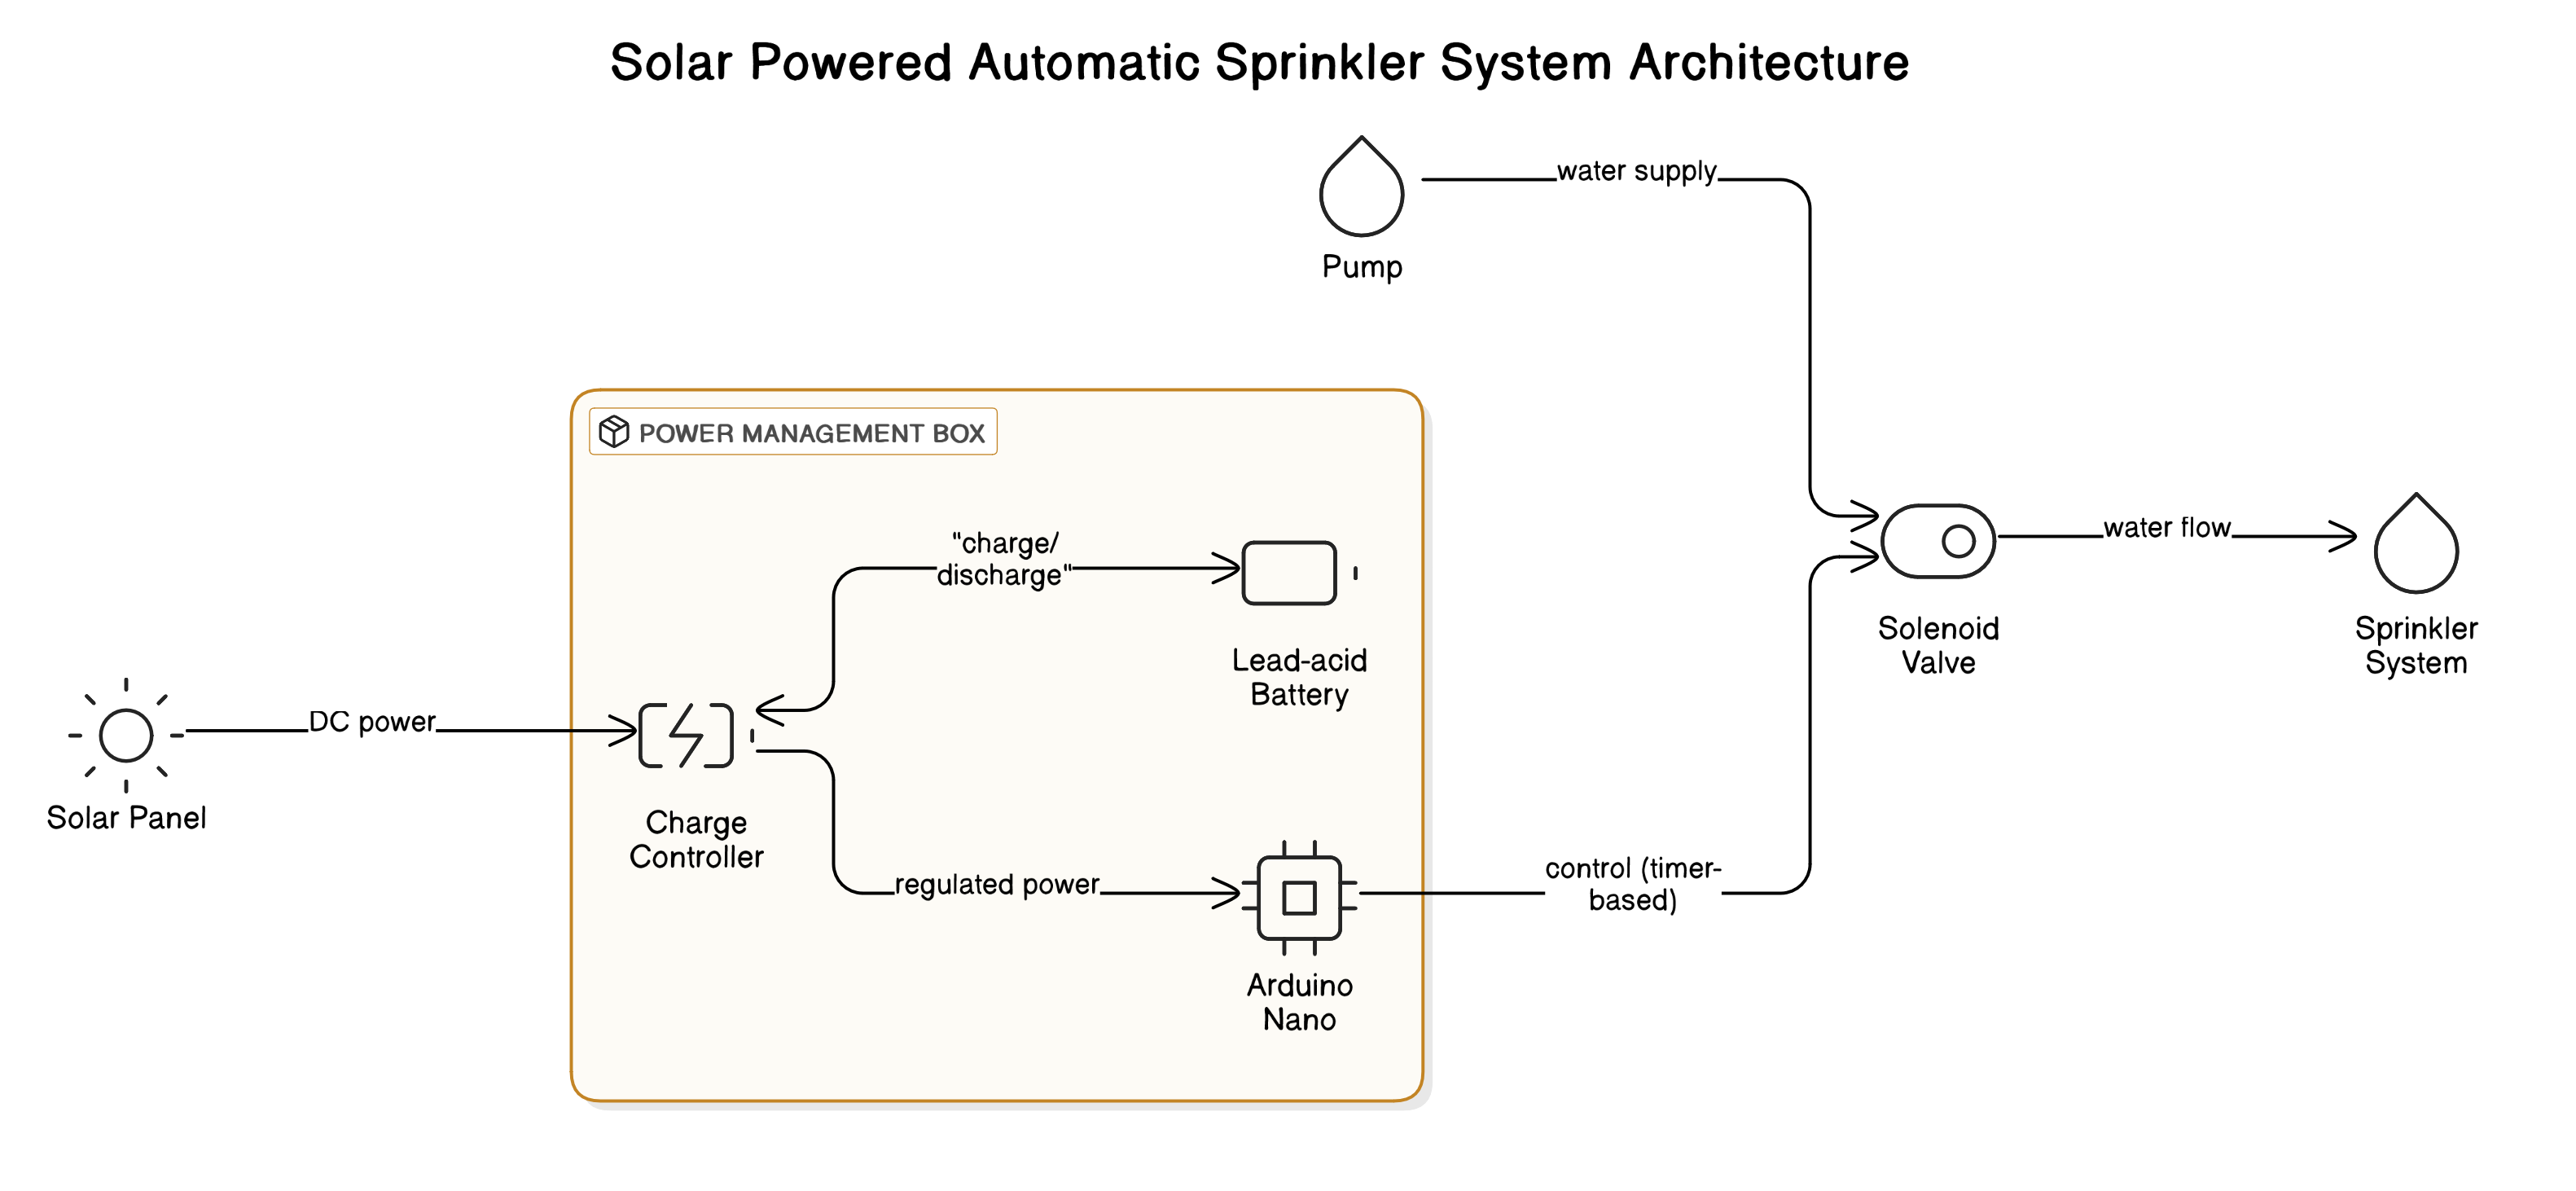
\includegraphics[width=1\textwidth]{imagenes/diagram.png}
      \caption{Diagrama de flujo del sistema de riego automatizado.}
      \label{fig:diagrama}
\end{figure}

\subsubsection{Diseño del Sistema}
Como se muestra en la Figura \ref{fig:diagrama}, se diseñó un sistema de riego automatizado utilizando energía solar como fuente principal. El sistema regará las plantas dos veces al día, a las 7:00 a.m. y a las 6:00 p.m., durante un periodo de 5 minutos cada vez. Todos los componentes electrónicos estarán protegidos en una caja IP-65 (Figura \ref{fig:caja} del Anexo), asegurando resistencia al agua y al polvo.

\subsubsection{Montaje del Sistema Eléctrico}
\begin{itemize}
      \item \textbf{Conexión del panel solar y la batería}: El panel solar (Figura \ref{fig:pane}) se conectará a la batería de 24V (Figura \ref{fig:bateria}) para garantizar su carga durante el día. Se recomienda utilizar un diodo en serie para evitar que la corriente vuelva al panel durante la noche.

      \item \textbf{Alimentación del Arduino Nano}: El Arduino Nano (Figura \ref{fig:arduino}) será alimentado directamente desde el controlador de carga (Figura \ref{fig:controlador}) para obtener 5V. El Arduino será el encargado de controlar la apertura y cierre de la electroválvula (Figura \ref{fig:electrovalve}) según el horario programado.

      \item \textbf{Control de la electroválvula}: La electroválvula será controlada a través de un driver de motor (Figura \ref{fig:motor}), que manejará el voltaje y la corriente adecuados para su funcionamiento. El Arduino enviará señales al driver para activar la electroválvula en los horarios especificados.
\end{itemize}

\subsubsection{Programación del Arduino Nano}
El Arduino Nano será programado para abrir y cerrar la electroválvula de forma automática a las horas definidas, implementando la lógica mostrada en el diagrama de flujo (Figura \ref{fig:diagrama}).

\subsubsection{Montaje del Sistema de Riego}
\begin{itemize}
      \item Instalación de la electroválvula en la tubería del sistema de riego para controlar el flujo de agua, como se muestra en las Figuras \ref{fig:sprinkler2} y \ref{fig:box} del Anexo.

      \item Conexión de mangueras para distribuir el agua desde la electroválvula hasta las plantas, siguiendo el diseño presentado en la Figura \ref{fig:diagrama}.

      \item Protección del sistema: Todos los componentes electrónicos (Arduino, driver de motor, batería) deben ser colocados en la caja IP-65 (Figura \ref{fig:caja}) para protegerlos de las condiciones ambientales externas.
\end{itemize}
\newpage
\section{Encuesta}
Para medir la opinión de los estudiantes de la sección primaria sobre la implementación de un tipo de energía limpia como lo es la luz solar, y su efectividad al ser utilizada para impulsar un sistema dentro de una institución educativa. Se aplicó una encuesta a 20 niños de quinto grado con edades entre 11 y 12 años.

\subsection{Resultados}
\begin{itemize}
      \item
            \textbf{Total survey participants}: 20 niños

      \item \textbf{¿Sabes qué es la energía renovable?}\\
            \textbf{Do you know what renewable energy is?}
            \begin{itemize}
                  \item Sí: 14 niños
                  \item No: 6 niños
                  \item Respuesta común (Sí): "Es la energía que se obtiene de fuentes naturales que no se agotan, como el sol y el viento."
            \end{itemize}

      \item \textbf{¿Se utiliza energía renovable en tu hogar?}\\
            \textbf{Is renewable energy used in your home?}
            \begin{itemize}
                  \item Sí: 8 niños
                  \item No: 10 niños
                  \item No estoy seguro: 2 niños
                  \item Respuesta común (No estoy seguro): "Creo que no tenemos paneles solares en casa."
            \end{itemize}

      \item \textbf{¿Los paneles solares requieren mantenimiento regular?}\\
            \textbf{Do solar panels require regular maintenance?}
            \begin{itemize}
                  \item Sí: 12 niños
                  \item No: 2 niños
                  \item No estoy seguro: 6 niños
                  \item Respuesta común (Sí): "Creo que sí, pero no sé exactamente qué tipo de mantenimiento necesitan."
            \end{itemize}

      \item \textbf{¿Es la energía solar una fuente de energía renovable?}\\
            \textbf{Is solar energy a renewable energy source?}
            \begin{itemize}
                  \item Sí: 20 niños
                  \item No: 0 niños
                  \item Respuesta común (Sí): "Sí, porque viene del sol y el sol nunca se acaba."
            \end{itemize}

      \item \textbf{¿Los paneles solares convierten la luz solar en electricidad?}\\
            \textbf{Do solar panels convert sunlight into electricity?}
            \begin{itemize}
                  \item Sí: 20 niños
                  \item No: 0 niños
                  \item Respuesta común (Sí): "Sí, eso es lo que hacen los paneles solares."
            \end{itemize}

      \item \textbf{¿Se puede almacenar la energía solar para su uso posterior?}\\
            \textbf{Can solar energy be stored for later use?}
            \begin{itemize}
                  \item Sí: 16 niños
                  \item No: 0 niños
                  \item No estoy seguro: 4 niños
                  \item Respuesta común (Sí): "Sí, en baterías especiales que guardan la energía para usarla después."
            \end{itemize}

      \item \textbf{¿Es la energía solar una alternativa más limpia a los combustibles fósiles?}\\
            \textbf{Is solar energy a cleaner alternative to fossil fuels?}
            \begin{itemize}
                  \item Sí: 18 niños
                  \item No: 0 niños
                  \item No estoy seguro: 2 niños
                  \item Respuesta común (Sí): "Sí, porque no contamina como el petróleo o el carbón."
            \end{itemize}

      \item \textbf{¿Pueden los sistemas solares ayudar a reducir las facturas de energía?}
            \\
            \textbf{Can solar systems help reduce energy bills?}
            \begin{itemize}
                  \item Sí: 16 niños
                  \item No: 2 niños
                  \item No estoy seguro: 2 niños
                  \item Respuesta común (Sí): "Sí, porque puedes usar la energía del sol en lugar de pagar por la electricidad."
            \end{itemize}

      \item \textbf{¿Es costosa la instalación de paneles solares?}
            \\
            \textbf{Is solar panel installation expensive?}
            \begin{itemize}
                  \item Sí: 14 niños
                  \item No: 2 niños
                  \item No estoy seguro: 4 niños
                  \item Respuesta común (Sí): "He oído que sí, al principio es cara, pero luego ahorras dinero."
            \end{itemize}

      \item \textbf{¿Es la energía solar una fuente inagotable?}
            \\
            \textbf{Is solar energy an inexhaustible source?}
            \begin{itemize}
                  \item Sí: 20 niños
                  \item No: 0 niños
                  \item Respuesta común (Sí): "Sí, porque el sol siempre estará ahí."
            \end{itemize}
\end{itemize}

\subsection{Conclusión de la Encuesta}
Los 20 niños del Club de Ecología de primaria tienen un conocimiento básico sobre la energía solar y las energías renovables. La mayoría sabe que la energía solar es una fuente inagotable y limpia, y entienden que los paneles solares convierten la luz del sol en electricidad. Aunque no todos están seguros si en sus hogares se utiliza energía renovable, reconocen los beneficios económicos y ambientales de la energía solar. Además, son conscientes de que los paneles solares requieren algún tipo de mantenimiento y que su instalación puede ser costosa inicialmente.




% \begin{center}
%       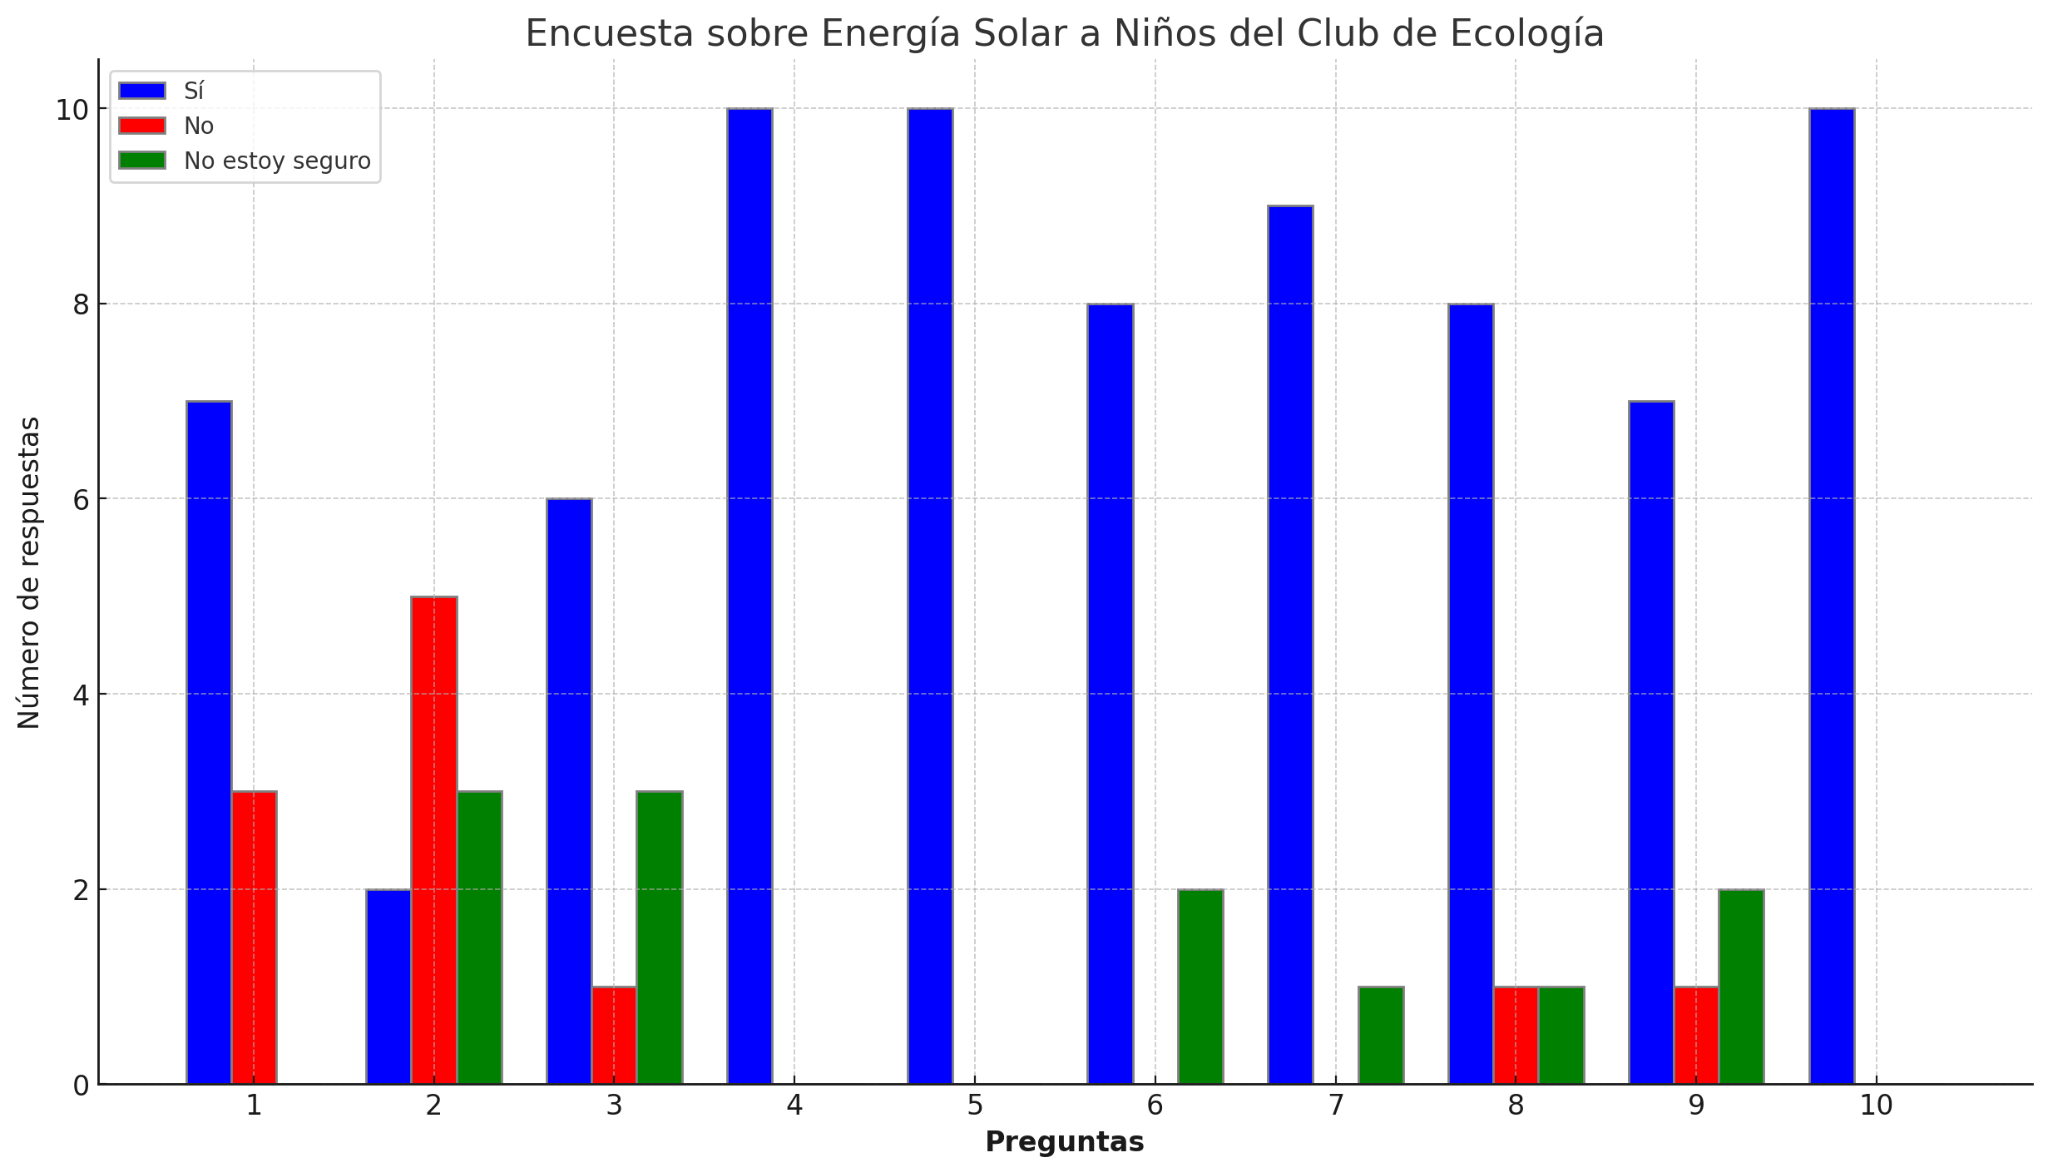
\includegraphics[width=0.5\textwidth]{imagenes/graph.png}
% \end{center}
\newpage
\section{Conclusión}
El acceso al agua potable es un desafío que ha acompañado a la humanidad a lo largo de la historia. En la actualidad, la crisis hídrica requiere soluciones innovadoras que permitan garantizar la disponibilidad y calidad del recurso de manera sostenible. En este sentido, Aqua Solar representa una propuesta tecnológica viable y eficaz, capaz de integrar energía solar en sistemas de abastecimiento de agua para comunidades con una infraestructura en un ecosistema de condiciones adversas.

Los hallazgos del proyecto demuestran que la energía fotovoltaica es una alternativa eficiente para la gestión del agua, reduciendo costos operativos y minimizando el impacto ambiental. A través de su implementación, se espera beneficiar a miles de personas, mejorando su calidad de vida y reduciendo los riesgos sanitarios asociados al consumo de agua no potable.

El impacto de Aqua Solar no se limita a sus beneficiarios directos, sino que sienta las bases para el desarrollo de nuevas estrategias de abastecimiento hídrico sostenible. A futuro, se plantea la posibilidad de expandir el proyecto a nivel regional, incorporando avances tecnológicos en almacenamiento de energía y automatización de los sistemas de distribución.

En definitiva, Aqua Solar demuestra que la combinación de tecnología y sostenibilidad es clave para enfrentar los retos actuales del acceso al agua. Su implementación no solo representa una solución innovadora, sino que también marca un precedente en la búsqueda de modelos sustentables que puedan replicarse a nivel global.


\newpage
\nocite{*}
\bibliography{referencias}  % Sin la extensión .bib
\bibliographystyle{apacite} % Estilo APA
\newpage
\section{Anexos}

\subsection*{Logo}
\begin{figure}[h!]
      \centering
      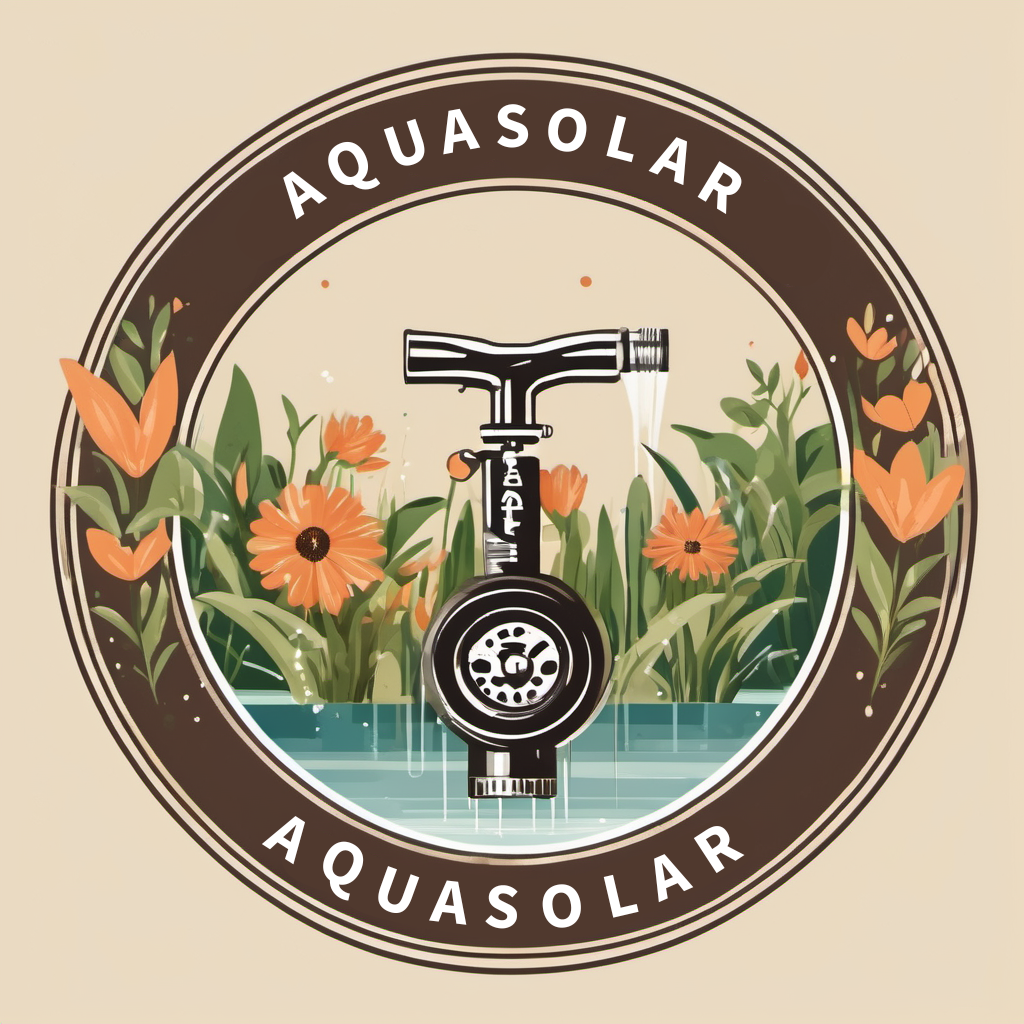
\includegraphics[width=0.5\textwidth]{imagenes/logo.png}
      \caption{Logo del proyecto}
      \label{fig:logo}
\end{figure}

\subsection*{Actividades}
\begin{figure}[h!]
      \centering
      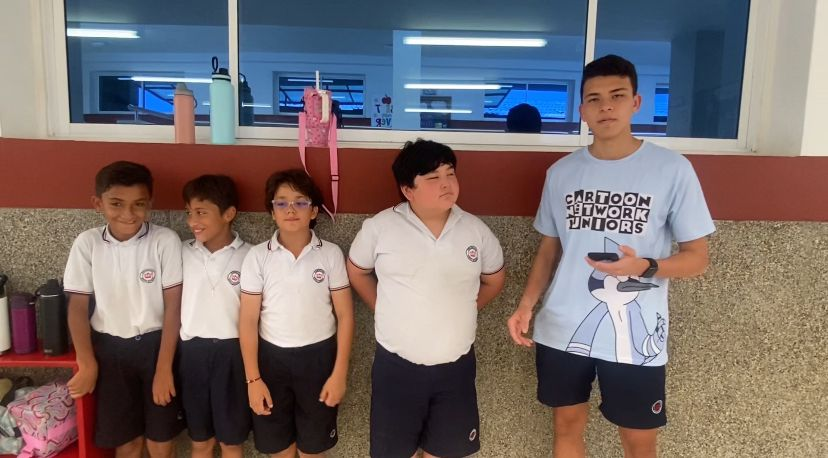
\includegraphics[width=0.5\textwidth]{imagenes/actividad1.jpg}
      \caption{Preparación del terreno para la instalación del sistema de riego}
      \label{fig:actividad1}
\end{figure}

\begin{figure}[h!]
      \centering
      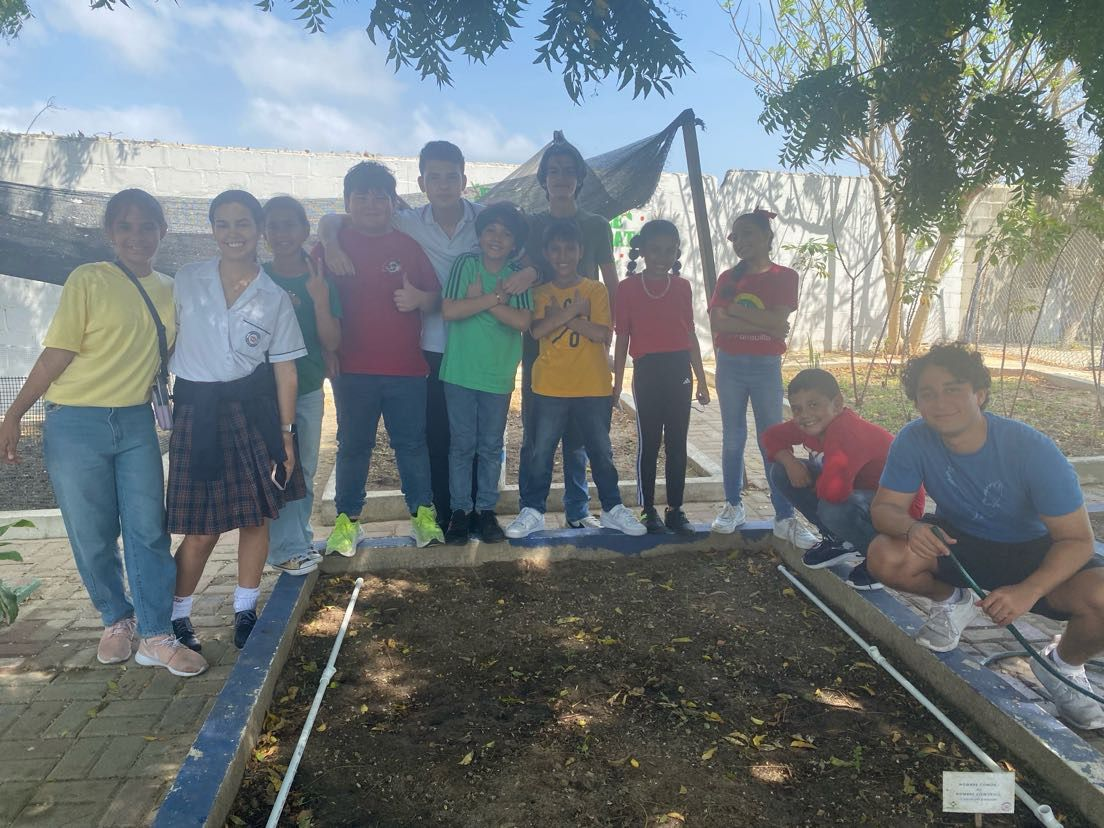
\includegraphics[width=0.5\textwidth]{imagenes/actividad2.jpg}
      \caption{Reforma del sistema de riego en la huerta escolar}
      \label{fig:actividad2}
\end{figure}

\begin{figure}[h!]
      \centering
      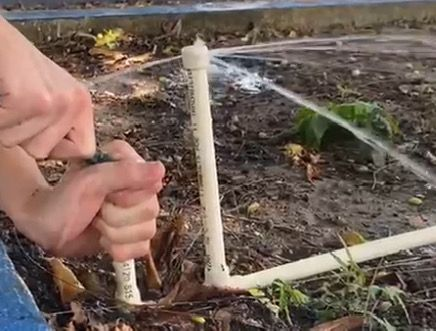
\includegraphics[width=0.5\textwidth]{imagenes/sprinkler.jpg}
      \caption{Participación del Club de Ecología de primaria en la reforma del sistema de riego}
      \label{fig:sprinkler}
\end{figure}

\begin{figure}[h!]
      \centering
      \begin{minipage}[b]{0.48\textwidth}
            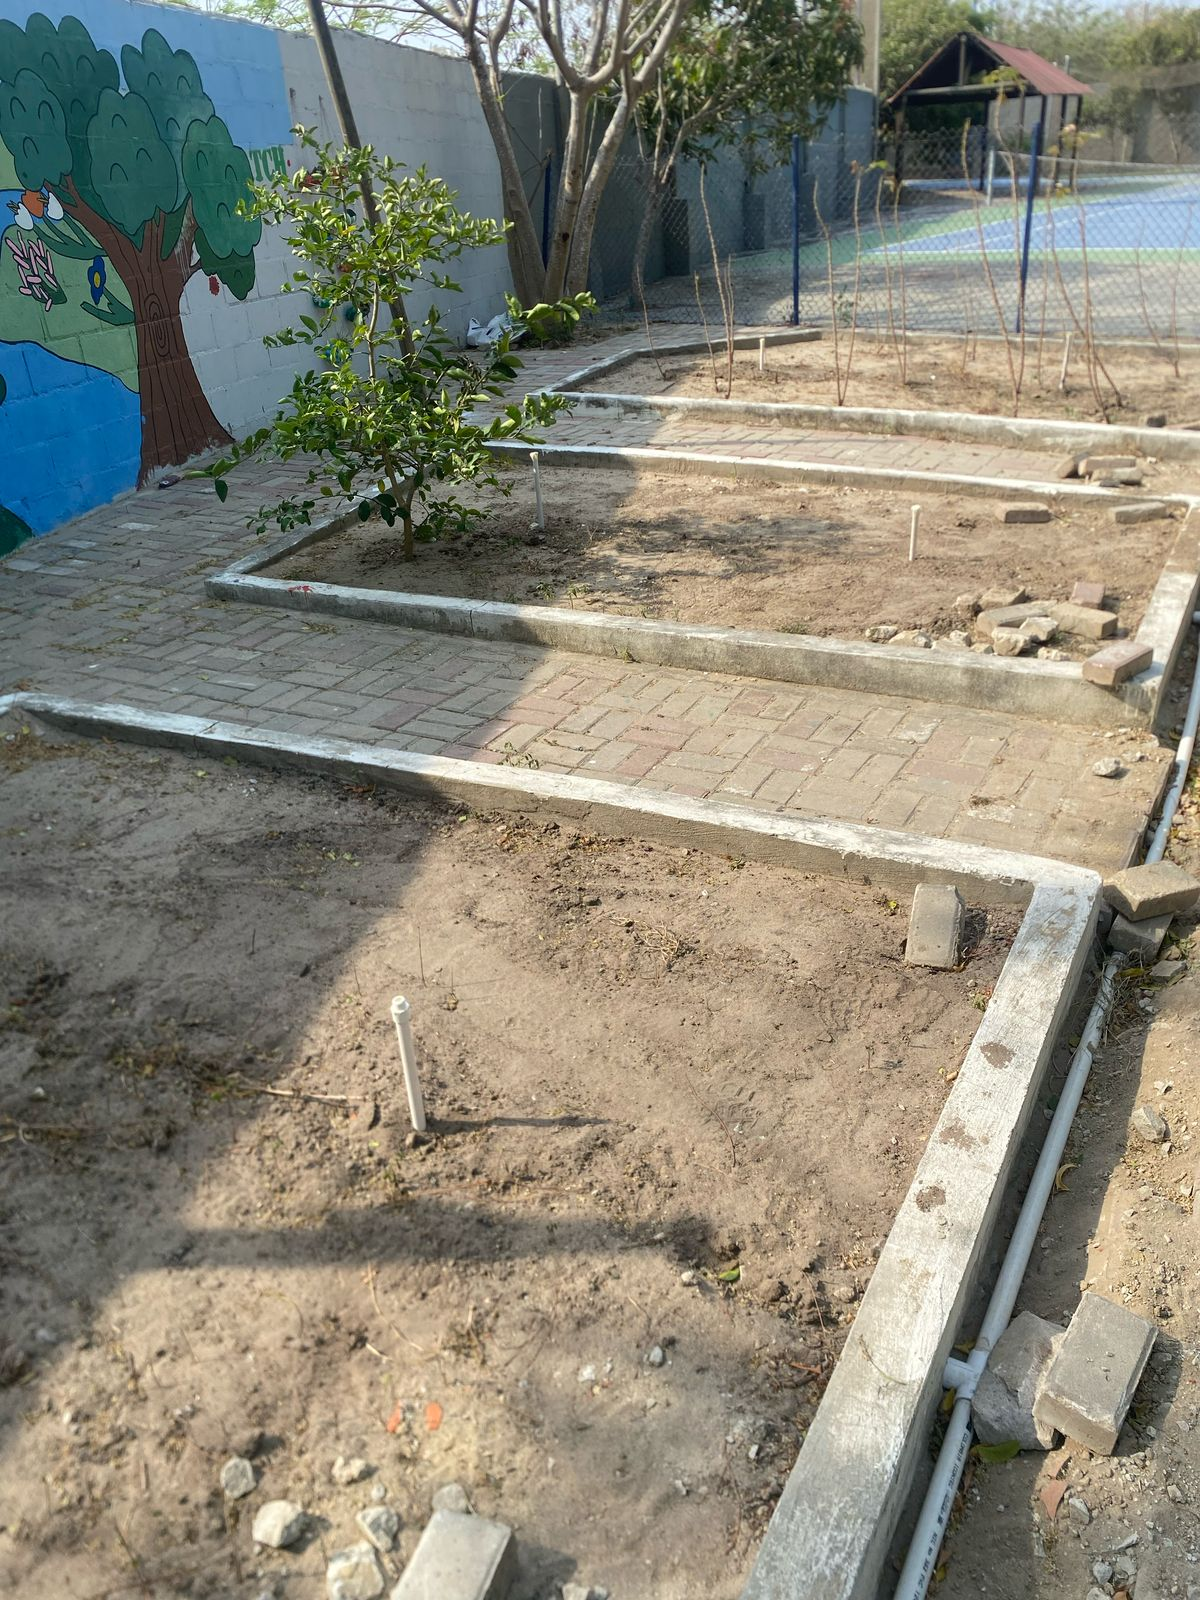
\includegraphics[width=\textwidth]{imagenes/sprinkler2.jpg}
            \caption{Instalación de la tubería}
            \label{fig:sprinkler2}
      \end{minipage}
      \hfill
      \begin{minipage}[b]{0.48\textwidth}
            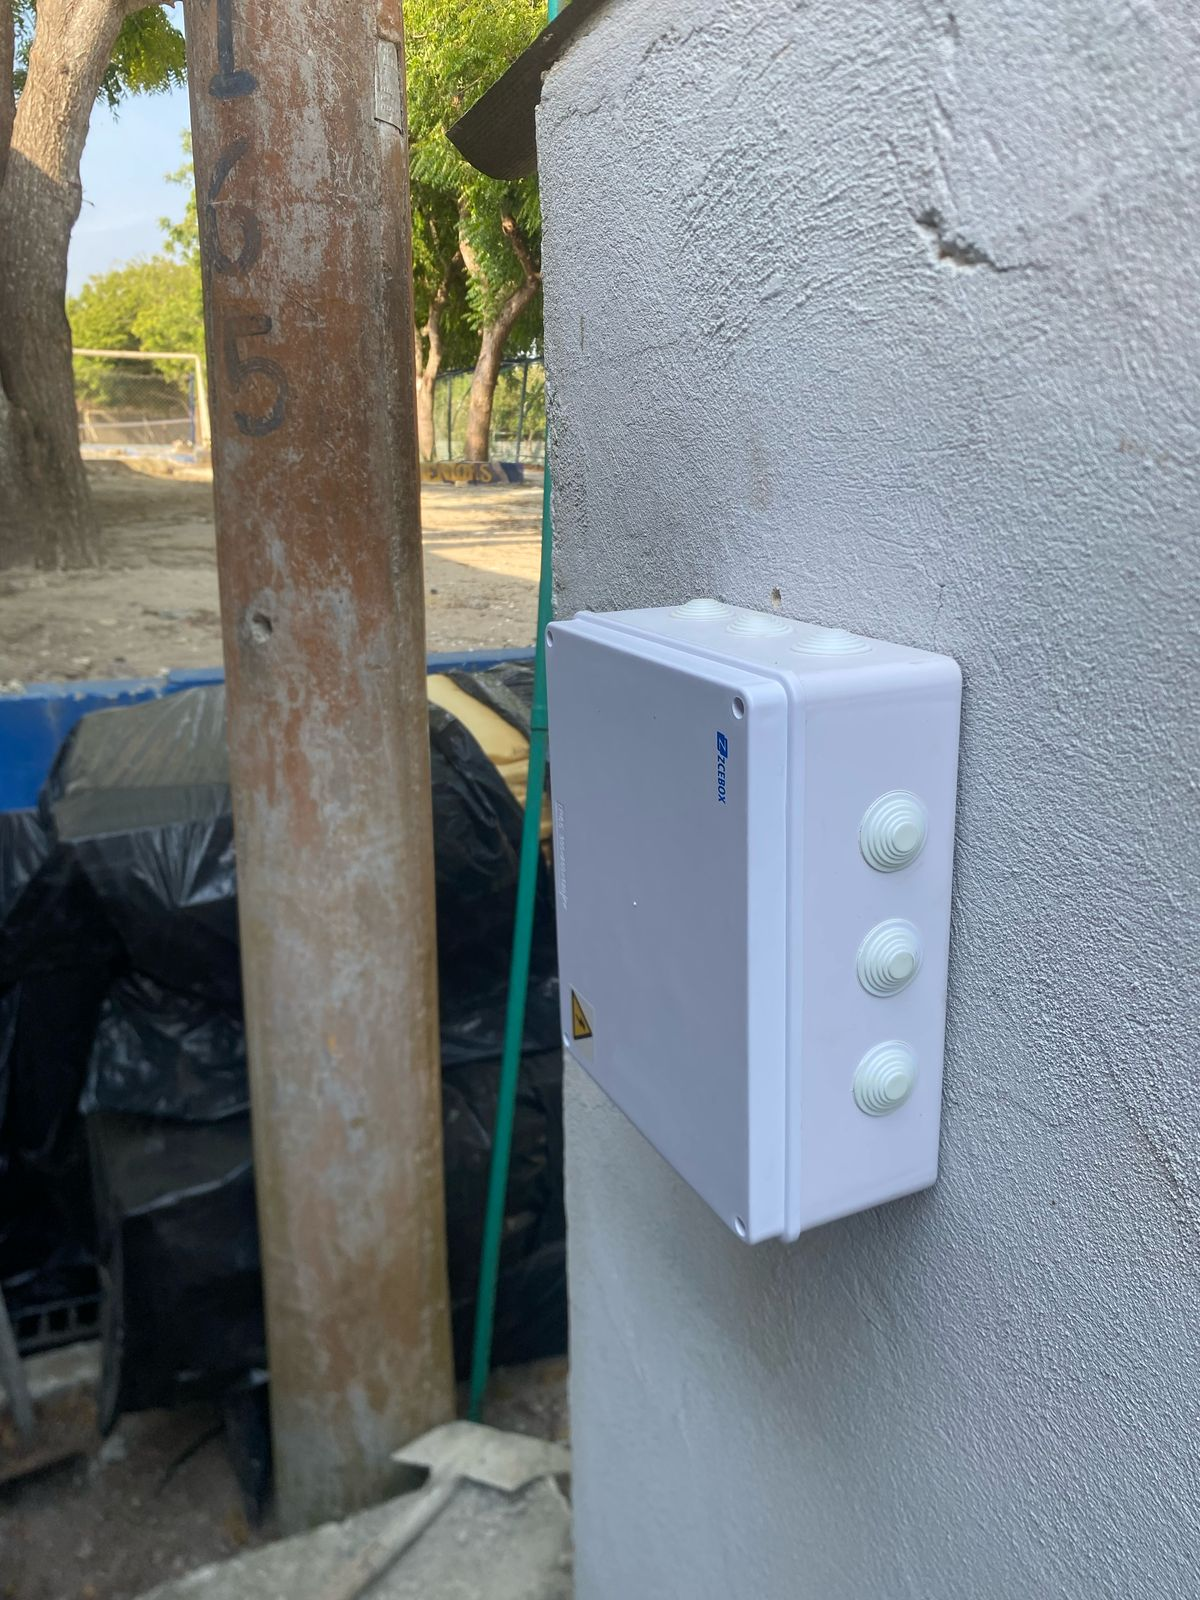
\includegraphics[width=\textwidth]{imagenes/box.jpg}
            \caption{Instalación de la caja IP-65}
            \label{fig:box}
      \end{minipage}
\end{figure}

\clearpage % Add page break to ensure separation

\subsection*{Materiales Utilizados}
\begin{figure}[h!]
      \centering
      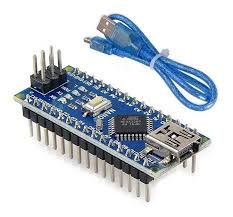
\includegraphics[width=0.3\textwidth]{imagenes/arduino.jpg}
      \caption{Arduino Nano}
      \label{fig:arduino}
\end{figure}

\begin{figure}[h!]
      \centering
      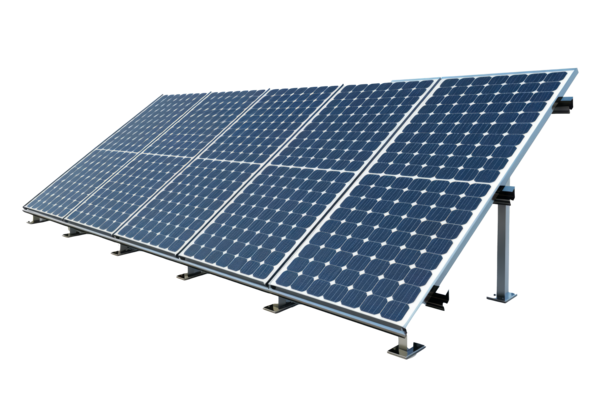
\includegraphics[width=0.3\textwidth]{imagenes/pane.png}
      \caption{Panel Solar}
      \label{fig:pane}
\end{figure}

\begin{figure}[h!]
      \centering
      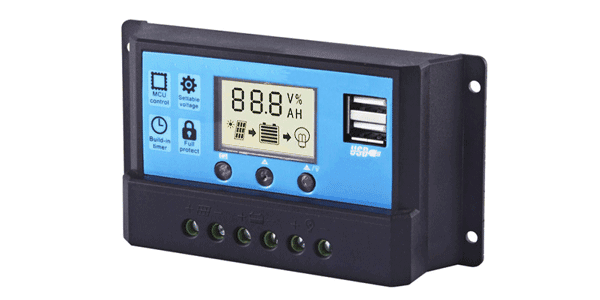
\includegraphics[width=0.3\textwidth]{imagenes/controlaor.png}
      \caption{Controlador de carga}
      \label{fig:controlador}
\end{figure}

\begin{figure}[h!]
      \centering
      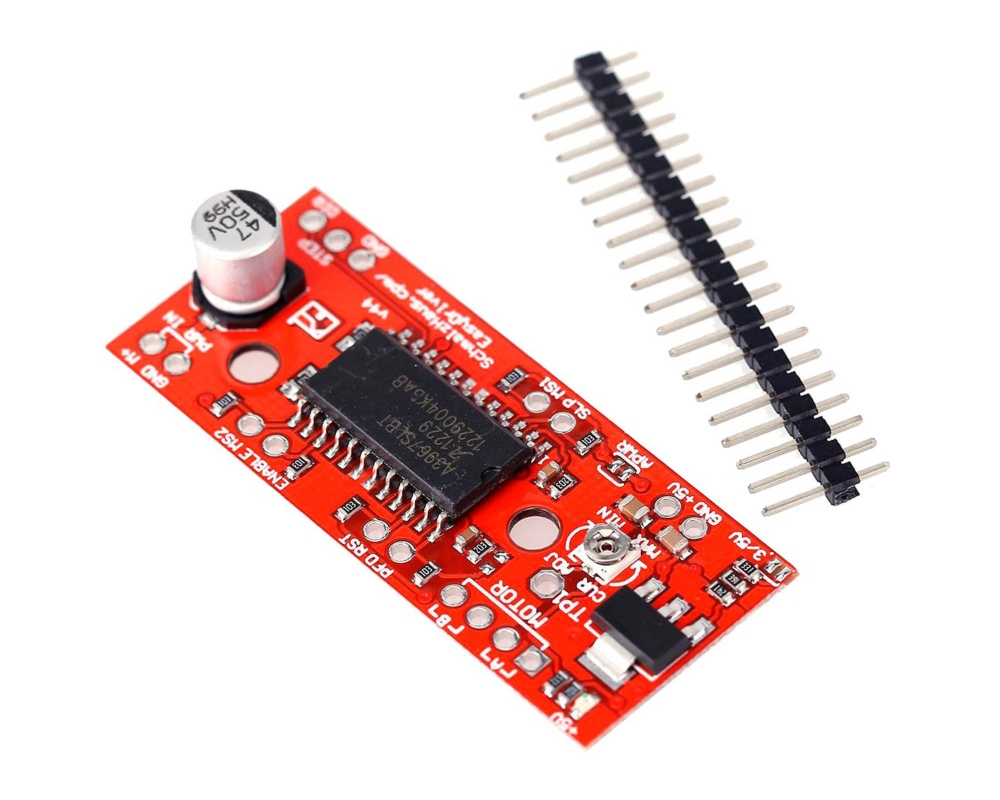
\includegraphics[width=0.3\textwidth]{imagenes/motor.png}
      \caption{Driver de motor}
      \label{fig:motor}
\end{figure}

\begin{figure}[h!]
      \centering
      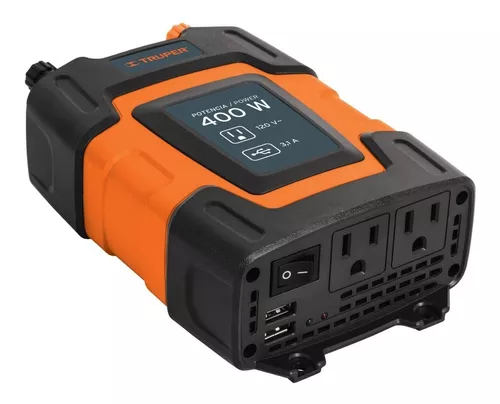
\includegraphics[width=0.3\textwidth]{imagenes/inversor.png}
      \caption{Inversor Truper - 200W}
      \label{fig:inversor}
\end{figure}

\begin{figure}[h!]
      \centering
      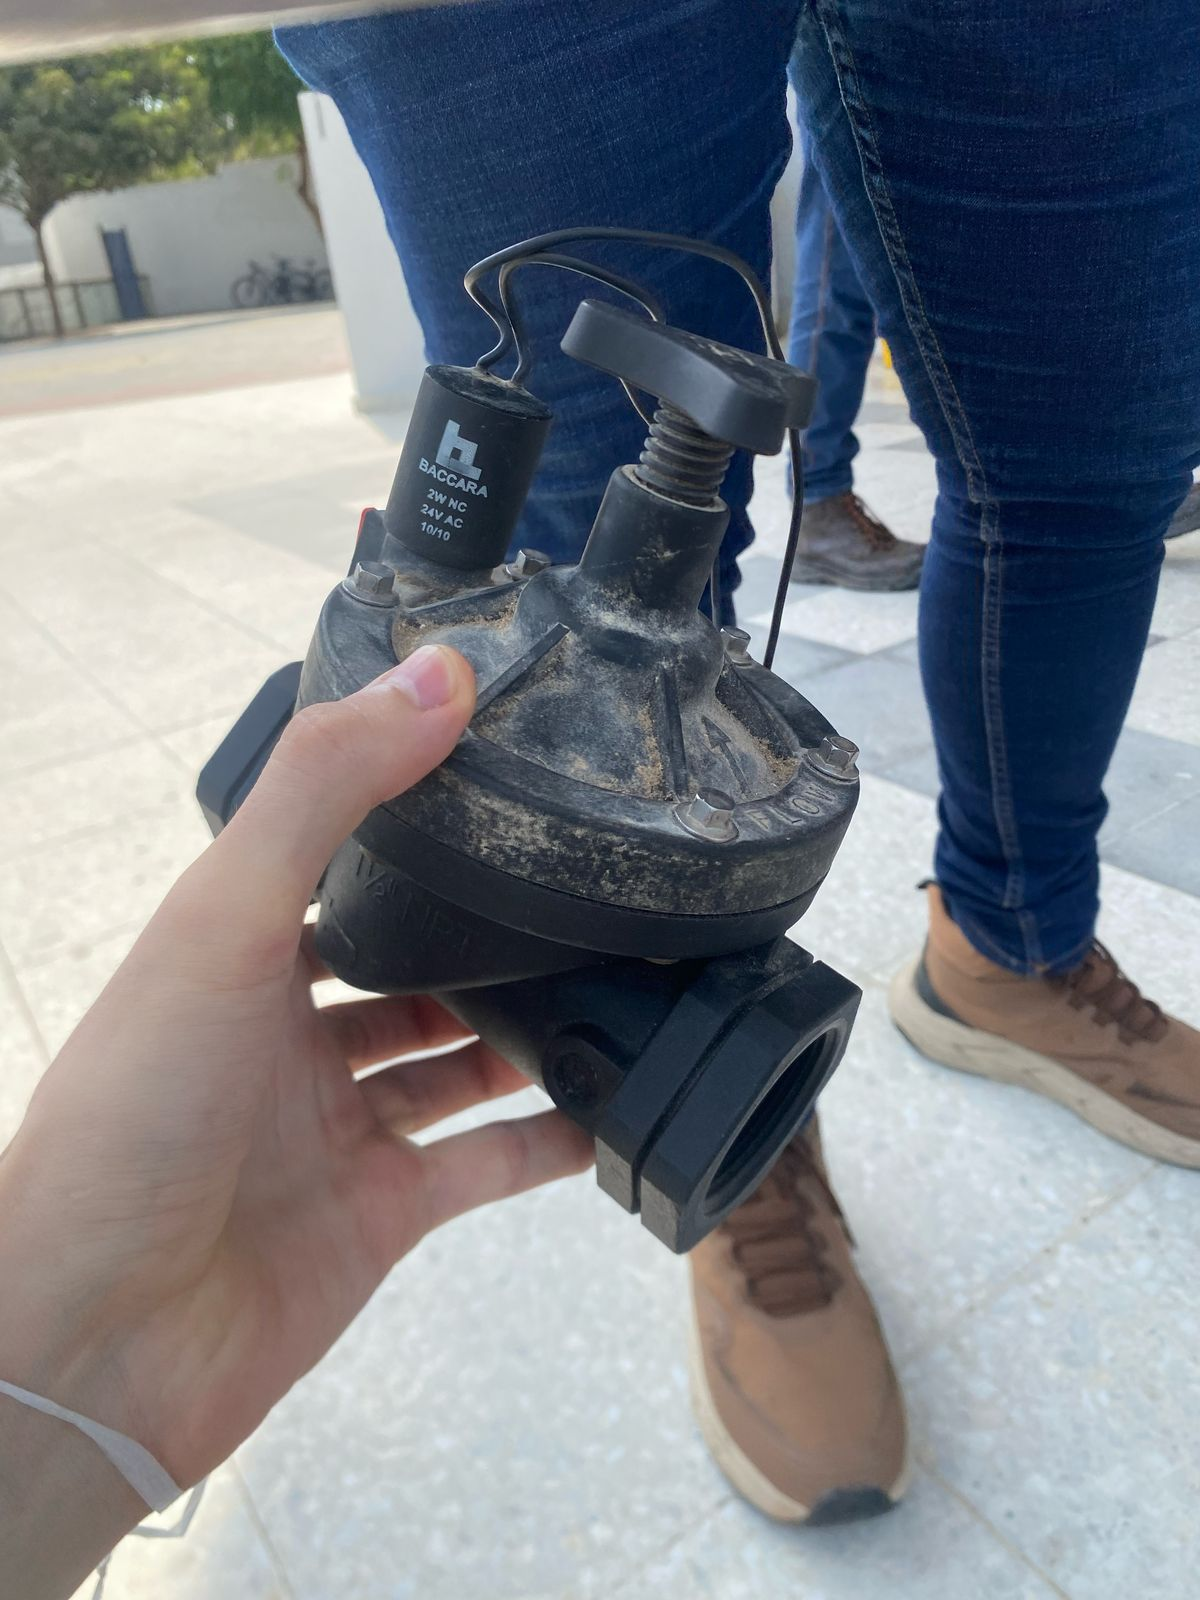
\includegraphics[width=0.3\textwidth]{imagenes/electrovalve2.jpg}
      \caption{Electroválvula}
      \label{fig:electrovalve}
\end{figure}

\begin{figure}[h!]
      \centering
      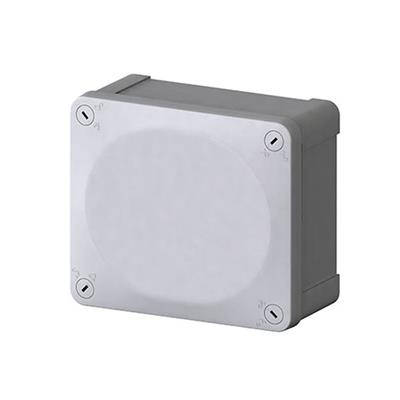
\includegraphics[width=0.3\textwidth]{imagenes/caja.png}
      \caption{Caja IP-65}
      \label{fig:caja}
\end{figure}

\begin{figure}[h!]
      \centering
      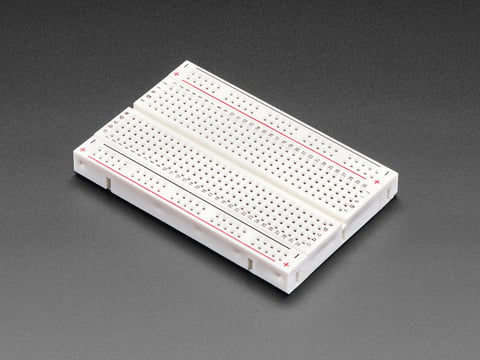
\includegraphics[width=0.3\textwidth]{imagenes/breadboard.png}
      \caption{Protoboard}
      \label{fig:breadboard}
\end{figure}

\begin{figure}[h!]
      \centering
      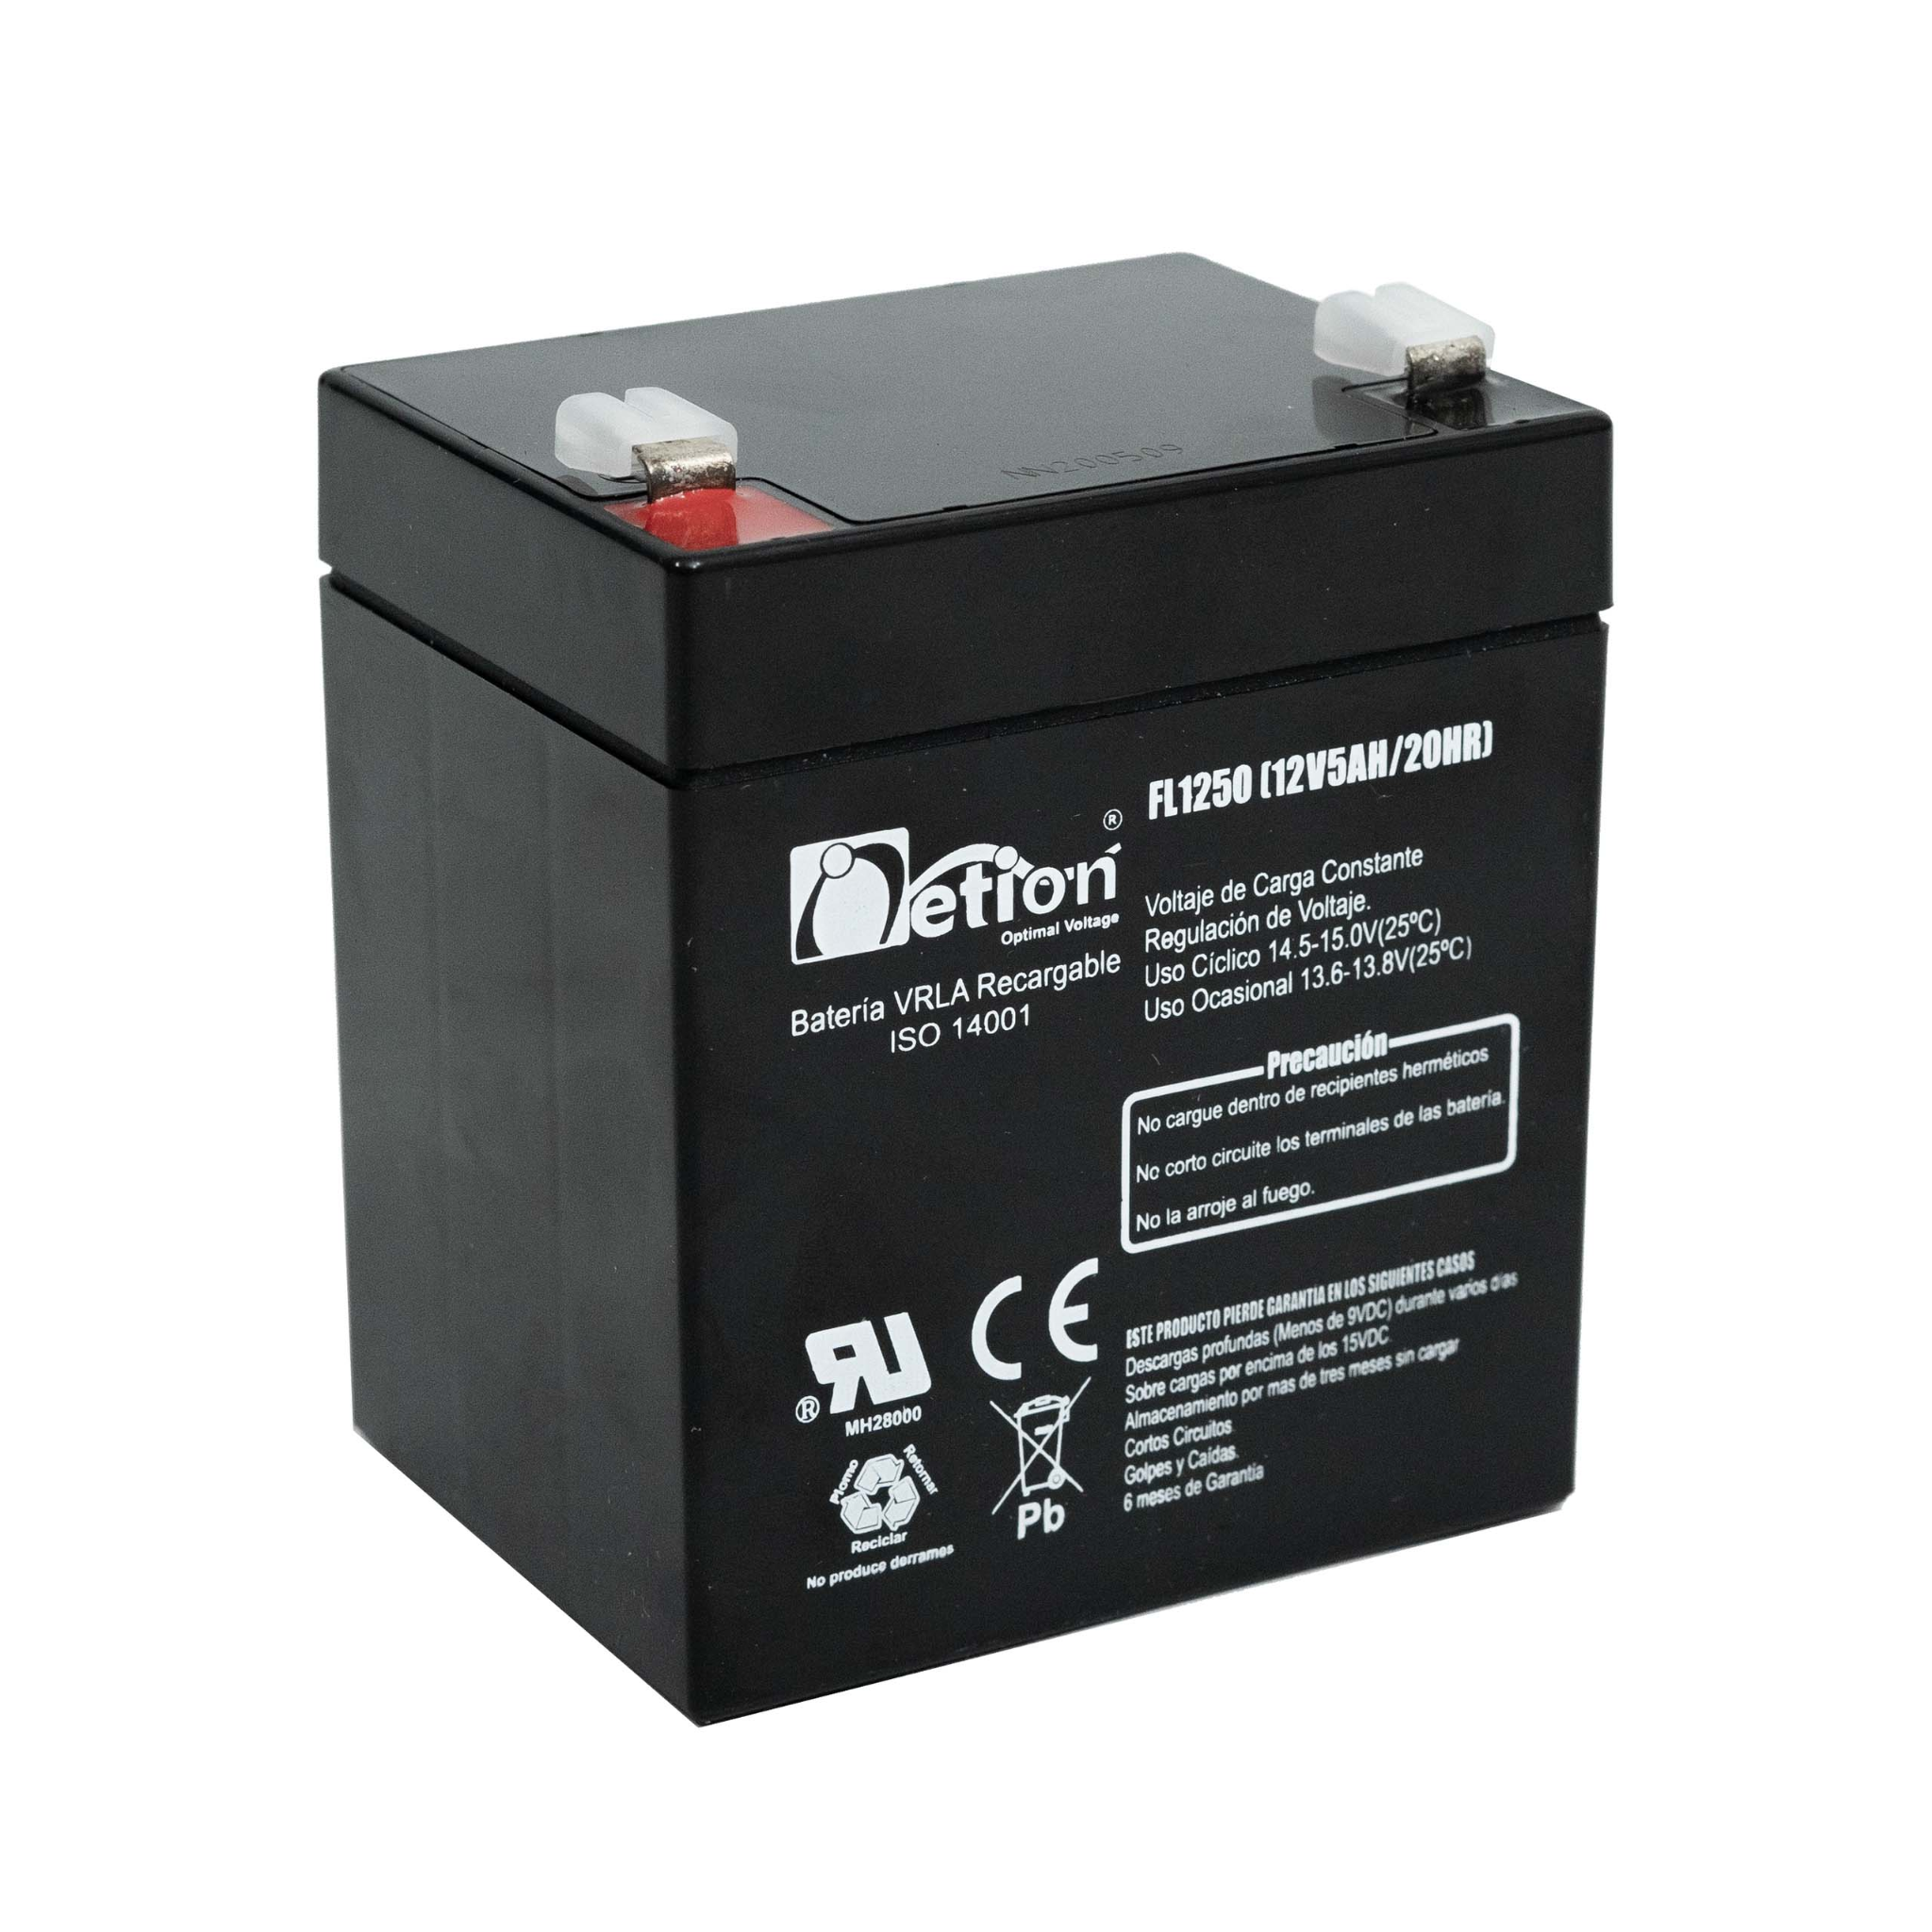
\includegraphics[width=0.3\textwidth]{imagenes/bateria.png}
      \caption{Batería 24V 5Ah/20HR}
      \label{fig:bateria}
\end{figure}
\end{document}